\chapter{Schémas électroniques}

L'électronique est une partie importante du robot et il est important de planifier en détail les schémas électriques avant d'imprimer les PCBs. Il est a noter que le robot fonctionne avec une batterie, donc tous les symboles de mise à la terre des schémas du robots font en fait référence au 0V de la batterie.

\section{Alimentation}

Le schéma électronique de l'alimentation de la figure \ref{fig:alim} possède un fusible d'entrée.
Sa fonction est de protéger les diverses composantes du robot.
Chacune des composantes est munie d'un interrupteur.
Des connecteurs MTA-156 sont utilisés pour faire le raccord entre le PCB d'alimentation et les dévolteurs.
En ce qui concerne le dévolteur de l'ordinateur embarqué, il est directement fixé au PCB d'alimentation.
Chacun des interrupteurs supporte un courant de 3A.
Des fils AWG 18 sont présents pour faire les différents raccords, ce qui est amplement suffisant pour l'ensemble des courants possibles et
ils permettent de minimiser la résistance. Un indicateur au LED est toujours pratique pour visualiser la présence de l'alimentation sur le PCB
provenant de la batterie Lipo. Des traces de 3mm sont utilisées pour limiter la présence de résistance inutile
et un plan de masse au-dessus du PCB a été mis en place.

\paragraph{}
Le shield de l'Arduino représenté à la figure \ref{fig:shield} permet un raccord facilité avec le pont H et les 4 moteurs roues.
Le PCB élimine un grand nombre de fils et il relie l'Arduino avec le drive de la bobine ainsi que pour le décodage du code Manchester.
Un plan de masse est présent sur l'ensemble du dessus du PCB.


\begin{landscape}
  \begin{figure}[ht]
    \centering
    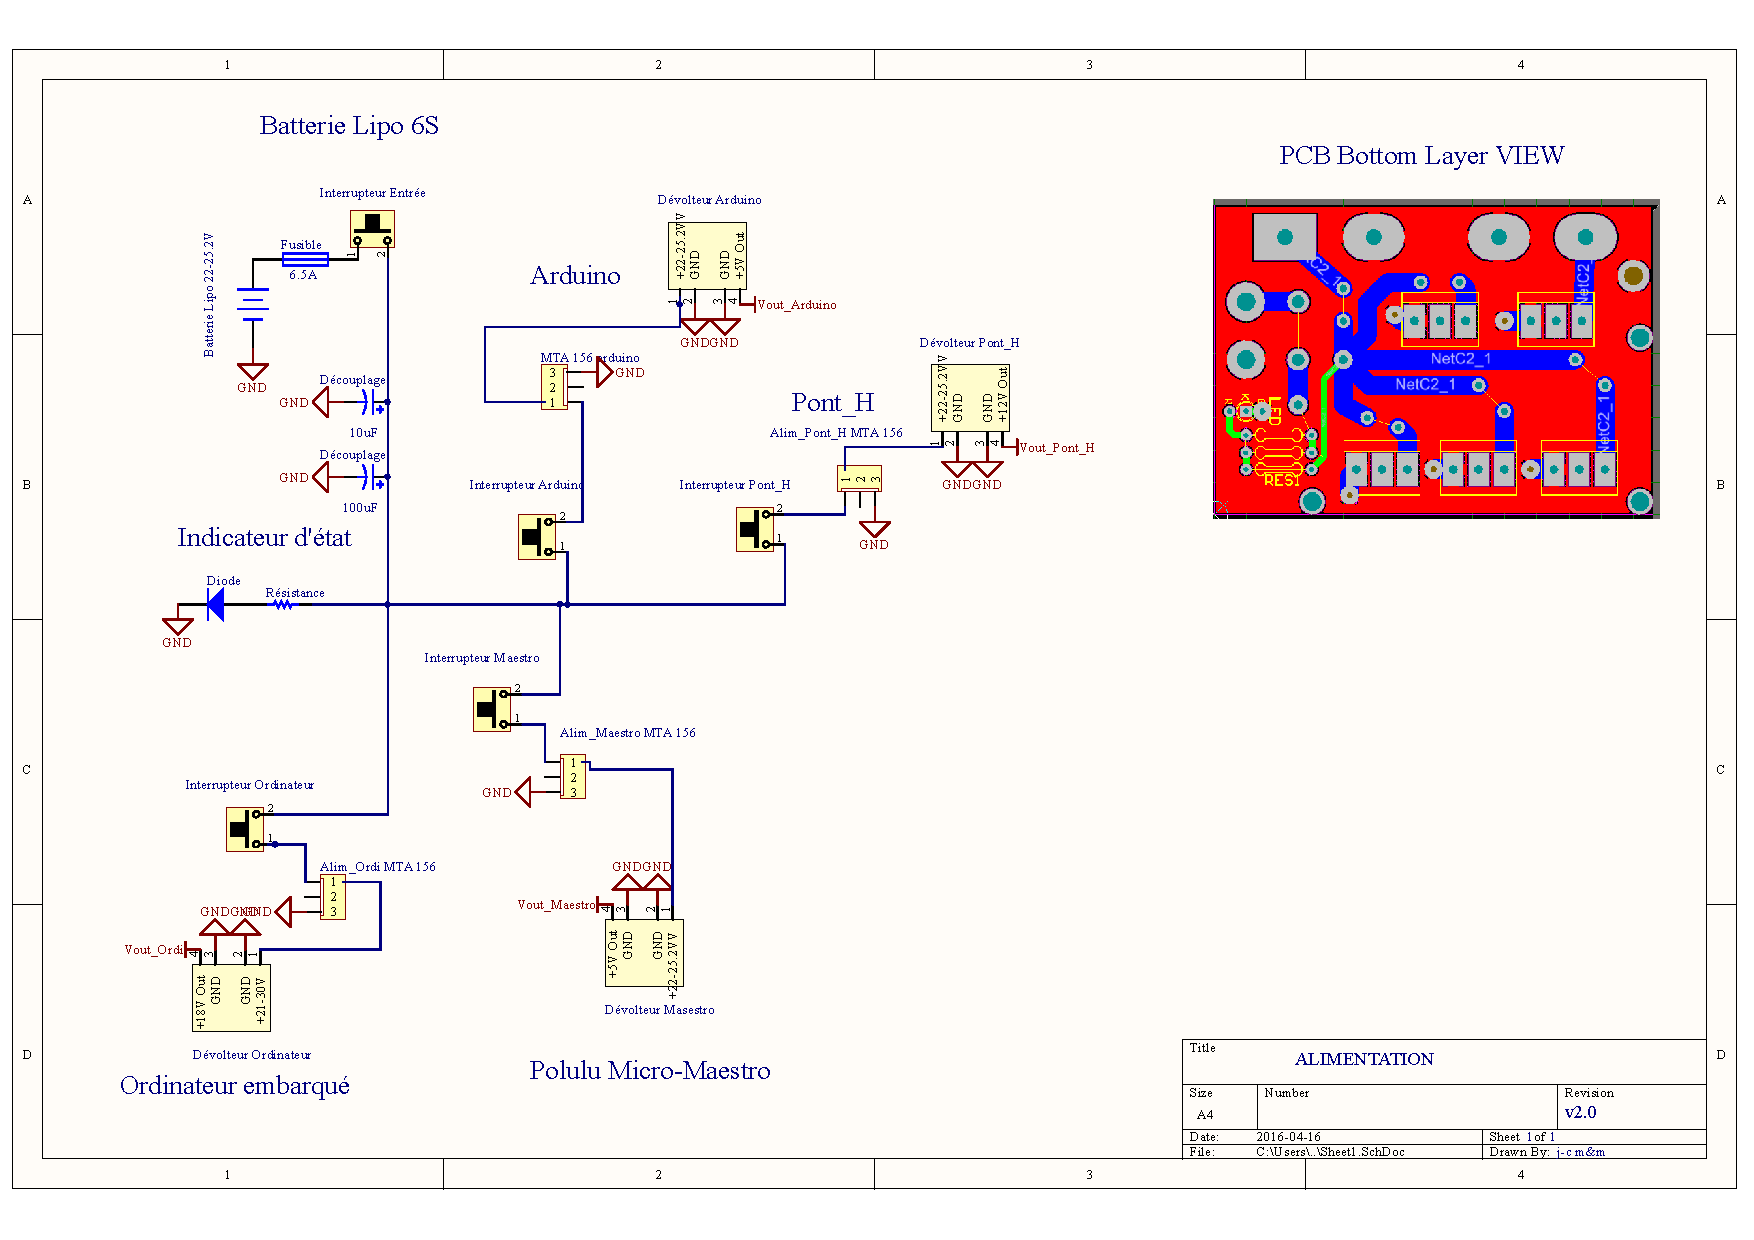
\includegraphics[scale=0.6]{resources/alim.pdf}
    \caption{Schéma électronique de l'alimentation}
    \label{fig:alim}
  \end{figure}

  \begin{figure}[ht]
    \centering
    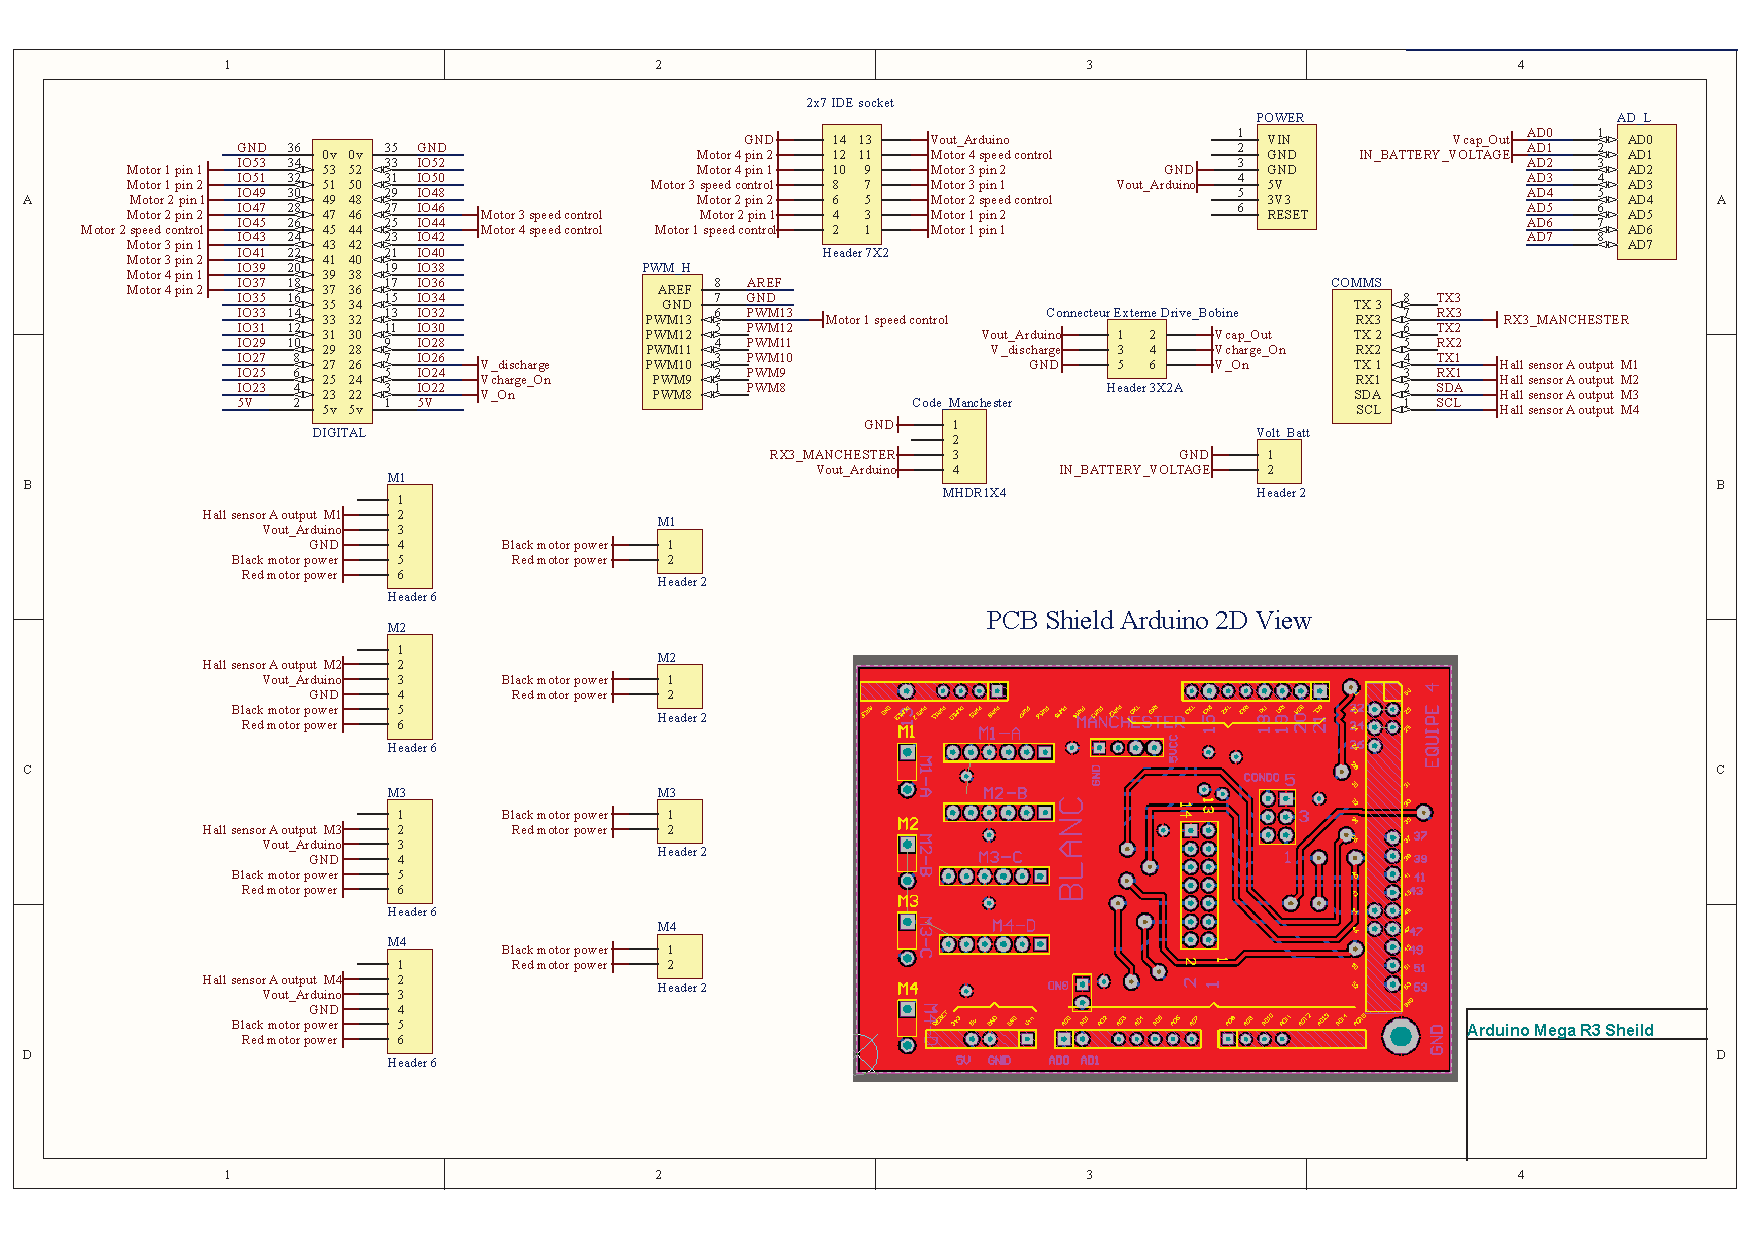
\includegraphics[scale=0.6]{resources/shield.pdf}
    \caption{Schéma électronique du shield de l'arduino}
    \label{fig:shield}
  \end{figure}
\end{landscape}

\section{Asservissement des moteurs}

L'asservissement est une partie très importante du robot, permettant de s'assurer que les déplacement des roues correspondent aux commandes envoyées peu importe les perturbations externes. Pour être fiable, une boucle de rétroaction doit être calibrée avec les bonnes constantes et doit s'éxécutée rapidement.
\paragraph{}
Afin d'asservir les mouvements du robot, chaque moteur possède une boucle de rétroaction en vitesse de type PI éxécutée à une fréquence de 20Hz. Pour connaitre la position des roues, les encodeurs à effet Hall sont utilisés. Puisque la direction des roues sont connues, un seul channel par encodeur est utilisé. À chaque front montant de l'encodeur, une interruption survient dans le microcontroleur, qui ne fait que décrémenter le nombre de \textit{ticks} restant. Ainsi, lorsque la boucle de rétroaction est éxécutée, il est possible de compter la différence de position depuis la dernière itération, et donc d'en déduire la vitesse actuelle des roues. 
\paragraph{}
Suite à plusieurs essais et expérimentations, il fut convenut que les constantes optimales pour la régulation des roues en vitesses sont $KI = 0.03$ et $KP = 0.05$. 
\paragraph{}
Parallèlement, une seconde boucle de rétroaction est utilisée pour s'assurer que le robot se déplace en ligne droite. En effet, lors des mouvements en ligne droite, les roues opposées ont toujours la même instruction. La deuxième boucle de rétroaction agit donc sur la différence des positions des roues opposées. Cette différence doit être de 0, et l'asservissement sert à ralentir une roue si elle prend de l'avance sur la roue opposée. Les constantes utilisées sur ce second asservissement sont $KI = 0.0075$ et $KP = 0.015$.
\section{Induction}

Le circuit représenté à la figure \ref{fig:induction} sert à induire un maximum de puissance au circuit de l'actionneur.
Un signal PWM est envoyé à partir du arduino de la station de base, ce dernier est amplifier par l'étage de puissance formé par les transistors.

\begin{figure}[ht]
  \centering
  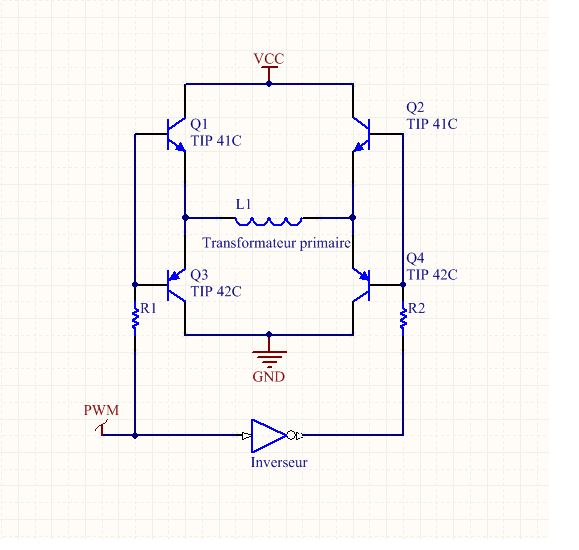
\includegraphics[scale=0.4]{resources/induction.png}
  \caption{Schéma électronique du circuit d'induction}
  \label{fig:induction}
\end{figure}

\section{Électroaimant}

\subsection{Chargeur du condensateur}

%%% Image chargeur
  \begin{figure}[ht]
    \centering
    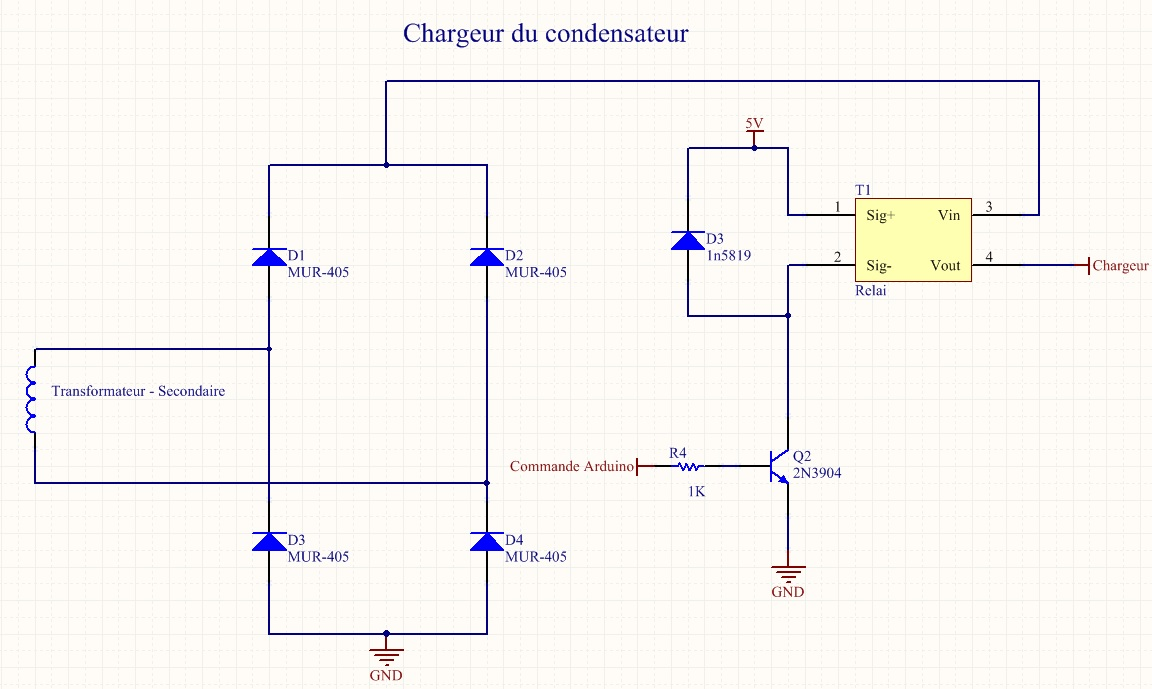
\includegraphics[scale=0.4]{resources/chargeur.jpg}
    \caption{Schéma électronique du chargeur du condensateur}
    \label{fig:chargeur}
  \end{figure}

La première étape de la charge du condensateur telle que représentée sur la figure \ref{fig:chargeur} est le redressage. On utilise un pont diodes pour redresser notre signal alternatif. Par la suite, on entre ce signal dans notre relai qui relie le pont de diodes aux condensateurs. Il s'agit de la pièce T1 sur le schéma. L'activation du relai est commandé par le arduino qui envoie un signal 0-5 volts dans la base du transistor qui \textit{drive} la bobine qui permet de fermer l'interrupteur du relai. Lorsqu'on active le relai, celui-ci devient un court-circuit et à cause que notre charge est inductive on charge à la vitesse maximale que le circuit d'induction peut fournir la puissance. En effet, si on applique une tension continu aux bornes d'un condensateur, on obtient un théorie un courant infini. Cependant, ici le courant est limité par le circuit d'induction.

\subsection{Électroaimant et voltage des condensateurs}

%%% image electroaimant_probage
  \begin{figure}[ht]
    \centering
    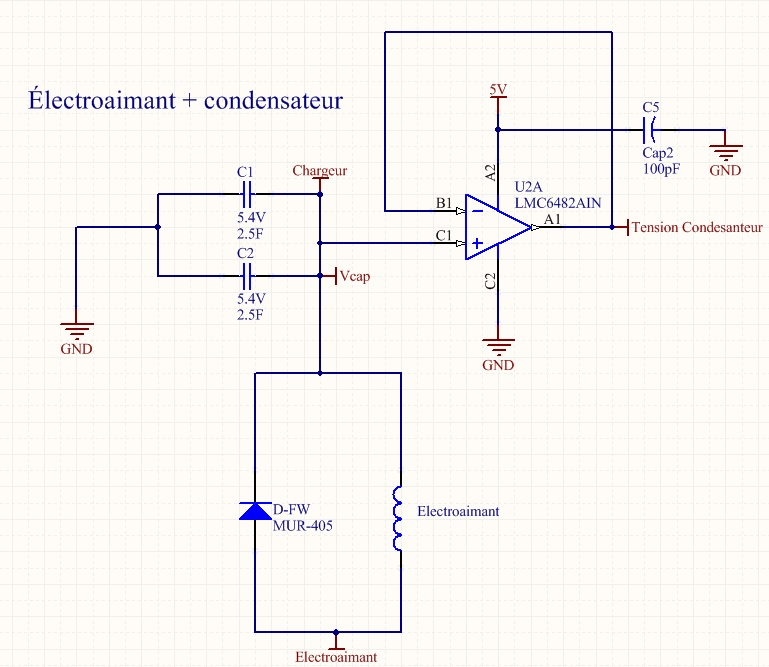
\includegraphics[scale=0.4]{resources/electroaimant_probage.jpg}
    \caption{Schéma électronique de l'électroaimant}
    \label{fig:electroaimant}
  \end{figure}
 
On observe sur la figure \ref{fig:electroaimant} la banque de condensateur qui sert à alimenter notre électroaimant. On mesure la tension des condensateurs avec un amplificateur opérationnel Rail-to-rail en mode suiveur. La sortie de cette amplificateur est fournit au convertisseur analogique-numérique du Arduino. On a mis un condensateur de découplage sur son alimentation pour limiter le bruit sur l'alimentation.

\subsection{Régulation du courant dans la bobine}

%%% image regulation_current
  \begin{figure}[ht]
    \centering
    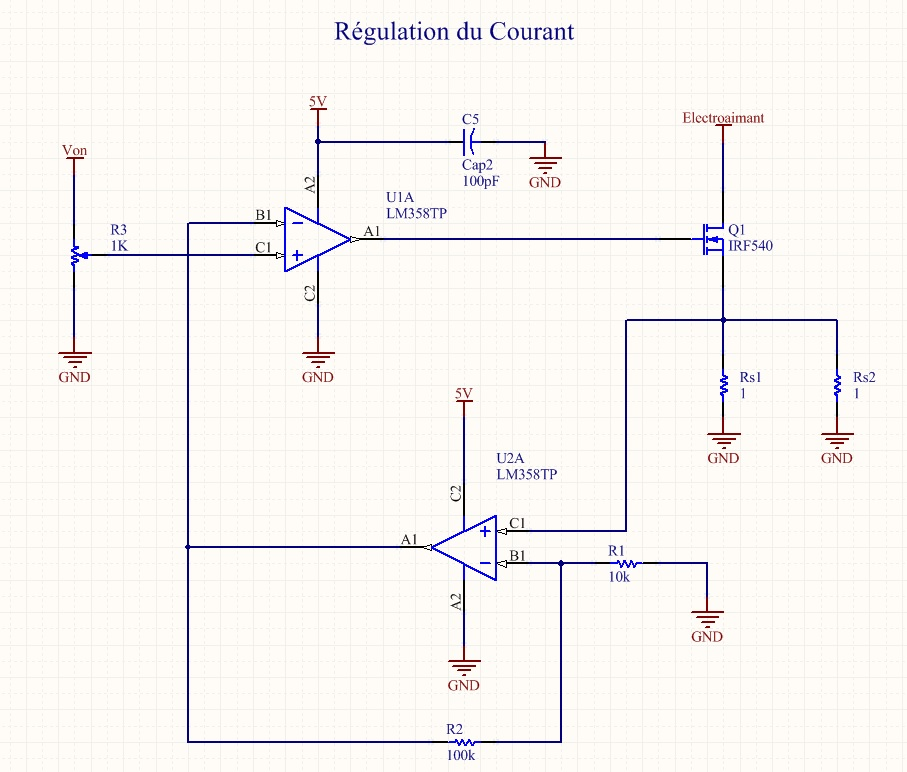
\includegraphics[scale=0.4]{resources/regulation_current.jpg}
    \caption{Schéma électronique de la régulation du courrant}
    \label{fig:reg_current}
  \end{figure}
Un régulateur analogique, tel que représenté à la figure \ref{fig:reg_current} est utilisé pour garder le courant constant dans la bobine. Pour ce faire, une source courant est créée avec un MOSFET, dont la consigne provient de l'erreur entre la commande et le courant mesuré dans le canal du MOSFET qui a été amplifié par une amplificateur en mode non-inverseur. La consigne est Von provient du arduino qui peut allumer ou fermer l'électroaimant. Encore ici, on a mis un condensateur de découplage sur l'alimentation de l'amplificateur.

\subsection{Décharge du condensateur}

%%% decharge
  \begin{figure}[ht]
    \centering
    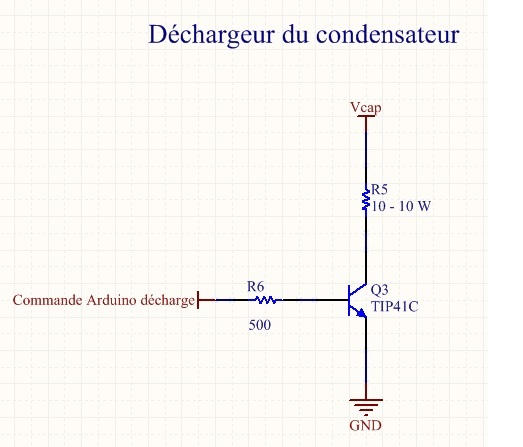
\includegraphics[scale=0.6]{resources/decharge.jpg}
    \caption{Schéma électronique de la décharge du condensateur}
    \label{fig:decharge}
  \end{figure}

Pour vider la charge dans le condensateur. On procède simplement en utilisant un transistor qui permet de vider la charge du condensateur dans une résistance de puissance, tel que sur le shéma de la figure \ref{fig:decharge}.
\section{Préhenseur}

Un préhenseur est requis afin de soulever le trésor et l'amener à destination.
Afin d'économiser la charge du condensateur, il faut miniser le temps où l'électroaimant est allumé.
Il est donc optimal de soulever le trésor à l'horizontal, dans une position où il repose sur une surface plate.

Pour ce faire, le préhenseur est constitué d'un arbre entraîné par un servo-moteur contrôllé par le pololu,
comme on peut voir sur la figure \ref{fig:lift_down}.
L'électroaimant destiné à prendre le trésor est fixé au milieu de l'arbre.
Lorsqu'un trésor est pris par le préhenseur, il est soulevé puis basculé contre un muret de bois comme sur la figure \ref{fig:lift_up}.
Il est alors possible de conserver le trésor sans qu'aucune puissance ne soit consommée.

\begin{figure}[ht]
  \centering
  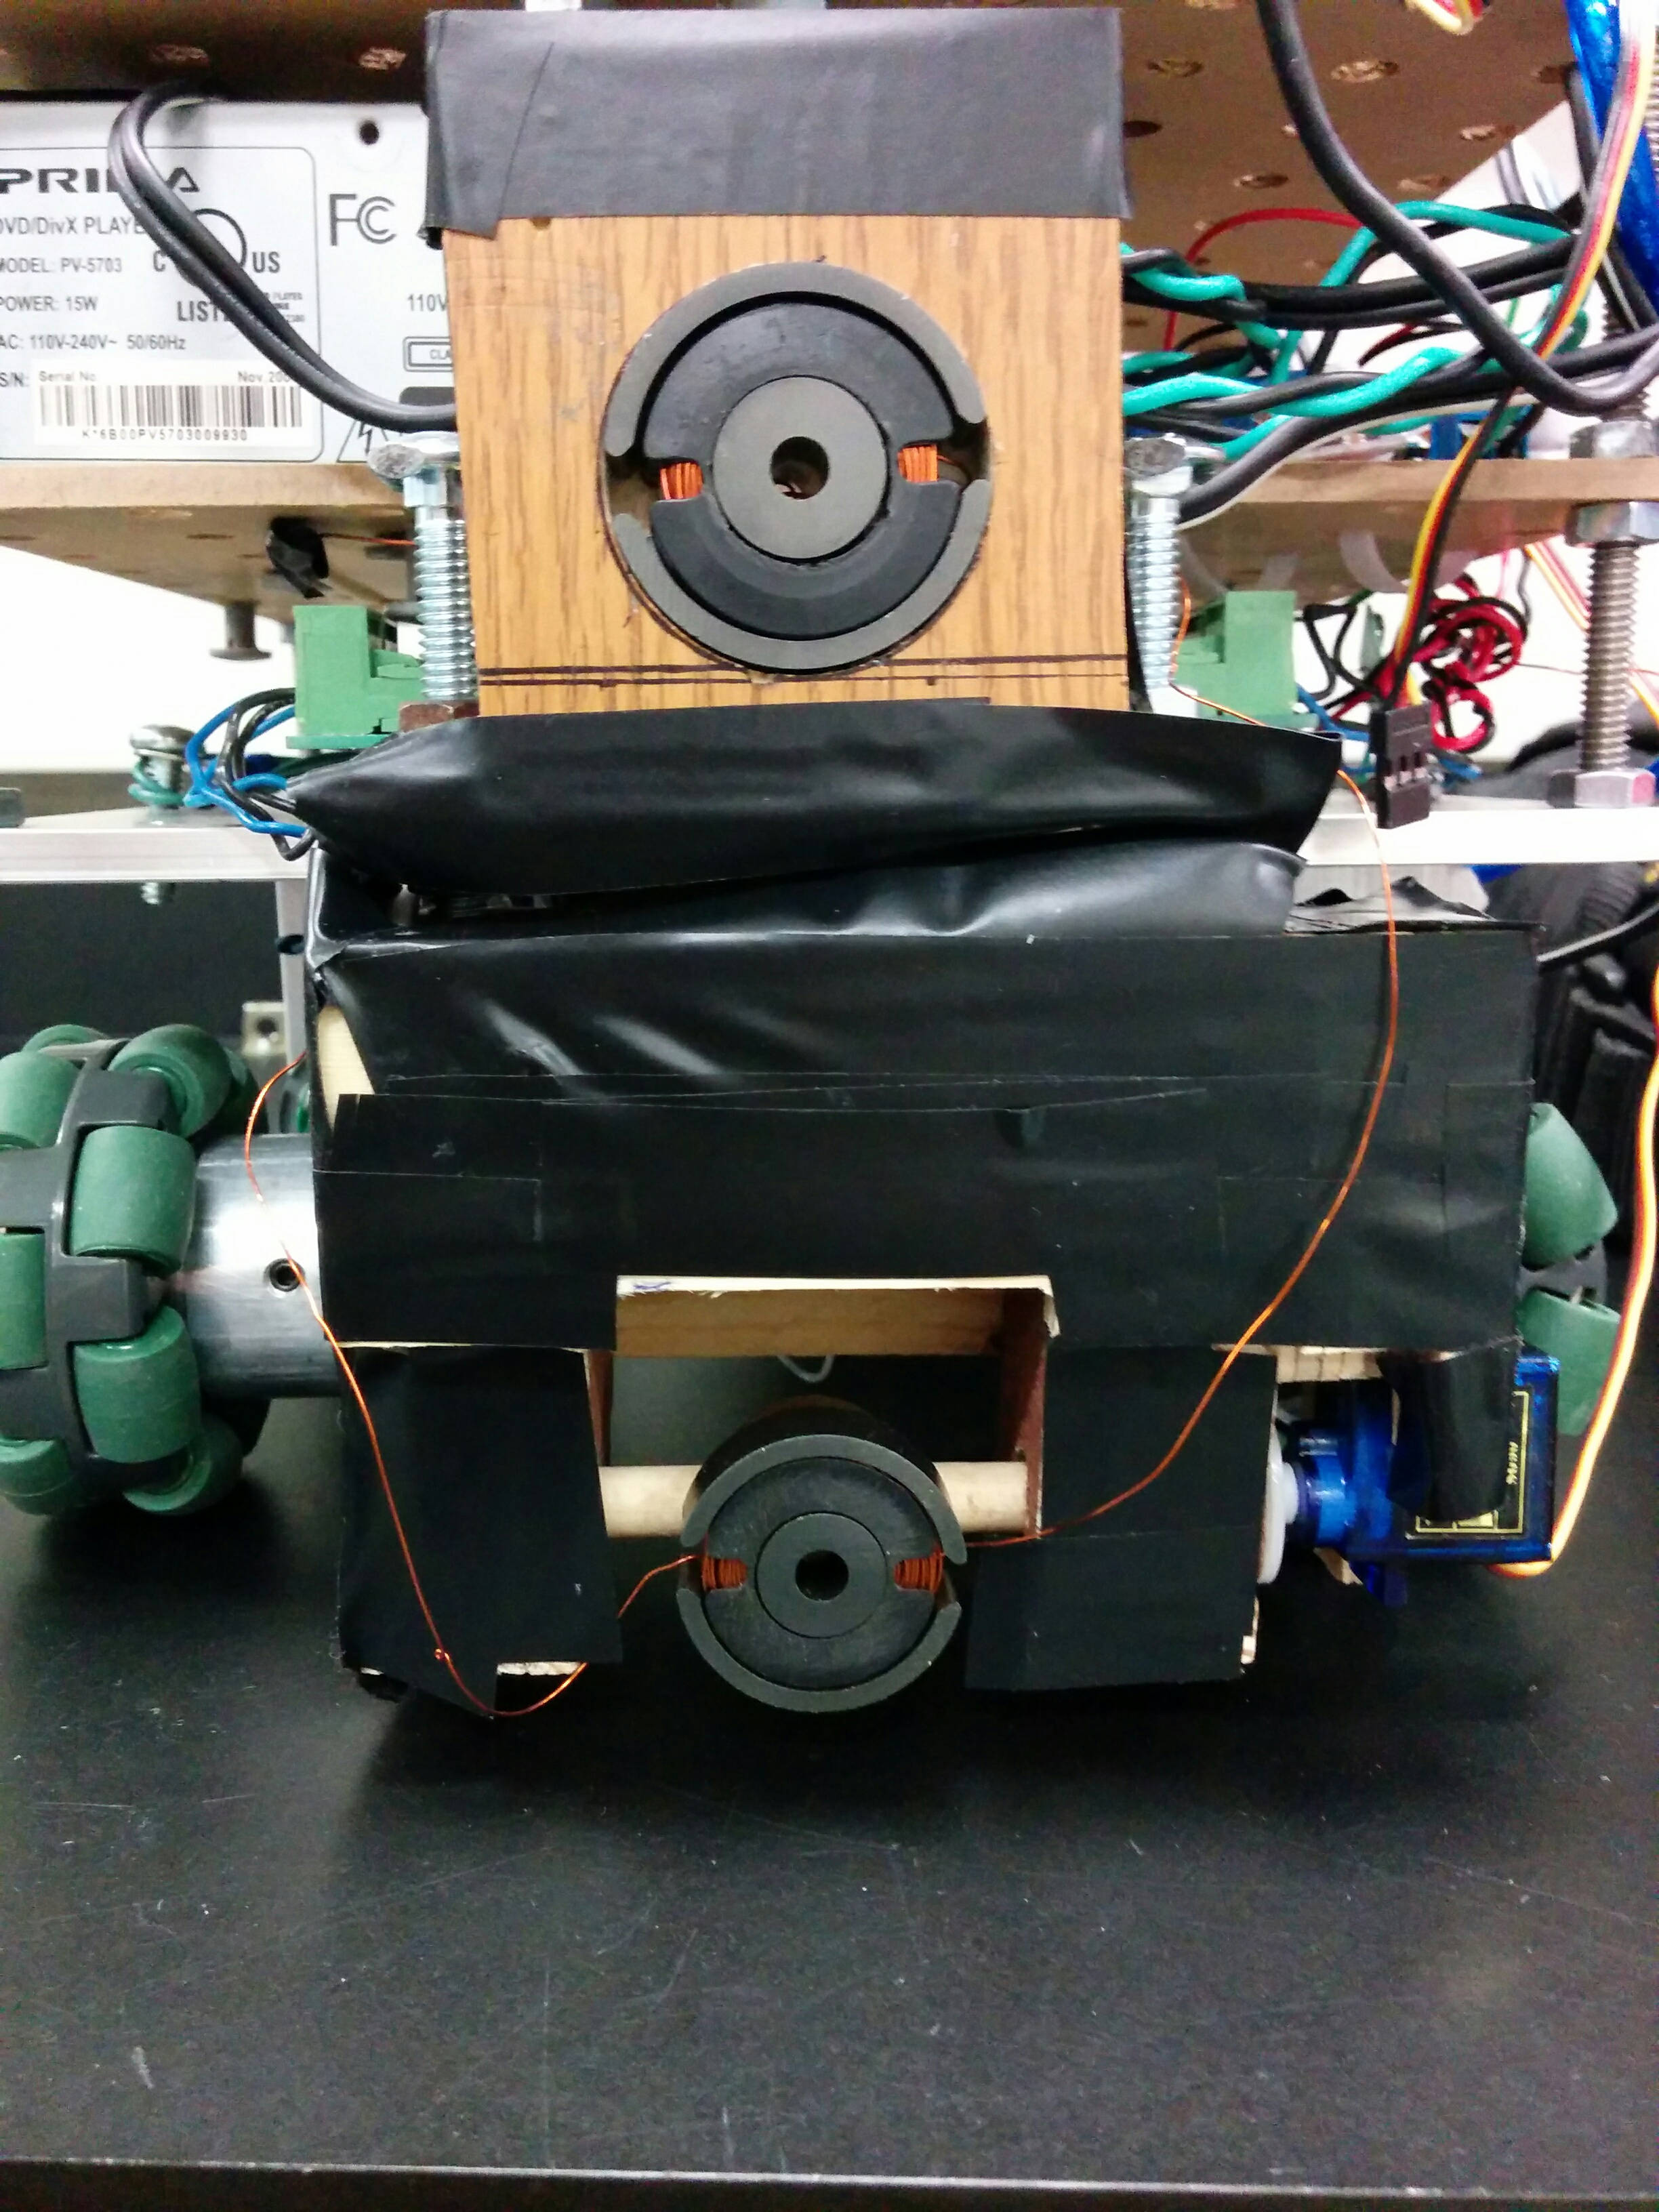
\includegraphics[scale=0.05]{resources/prehenseur_down.jpg}
  \caption{préhenseur en position de prise de trésor}
  \label{fig:lift_down}
\end{figure}

\begin{figure}[ht]
  \centering
  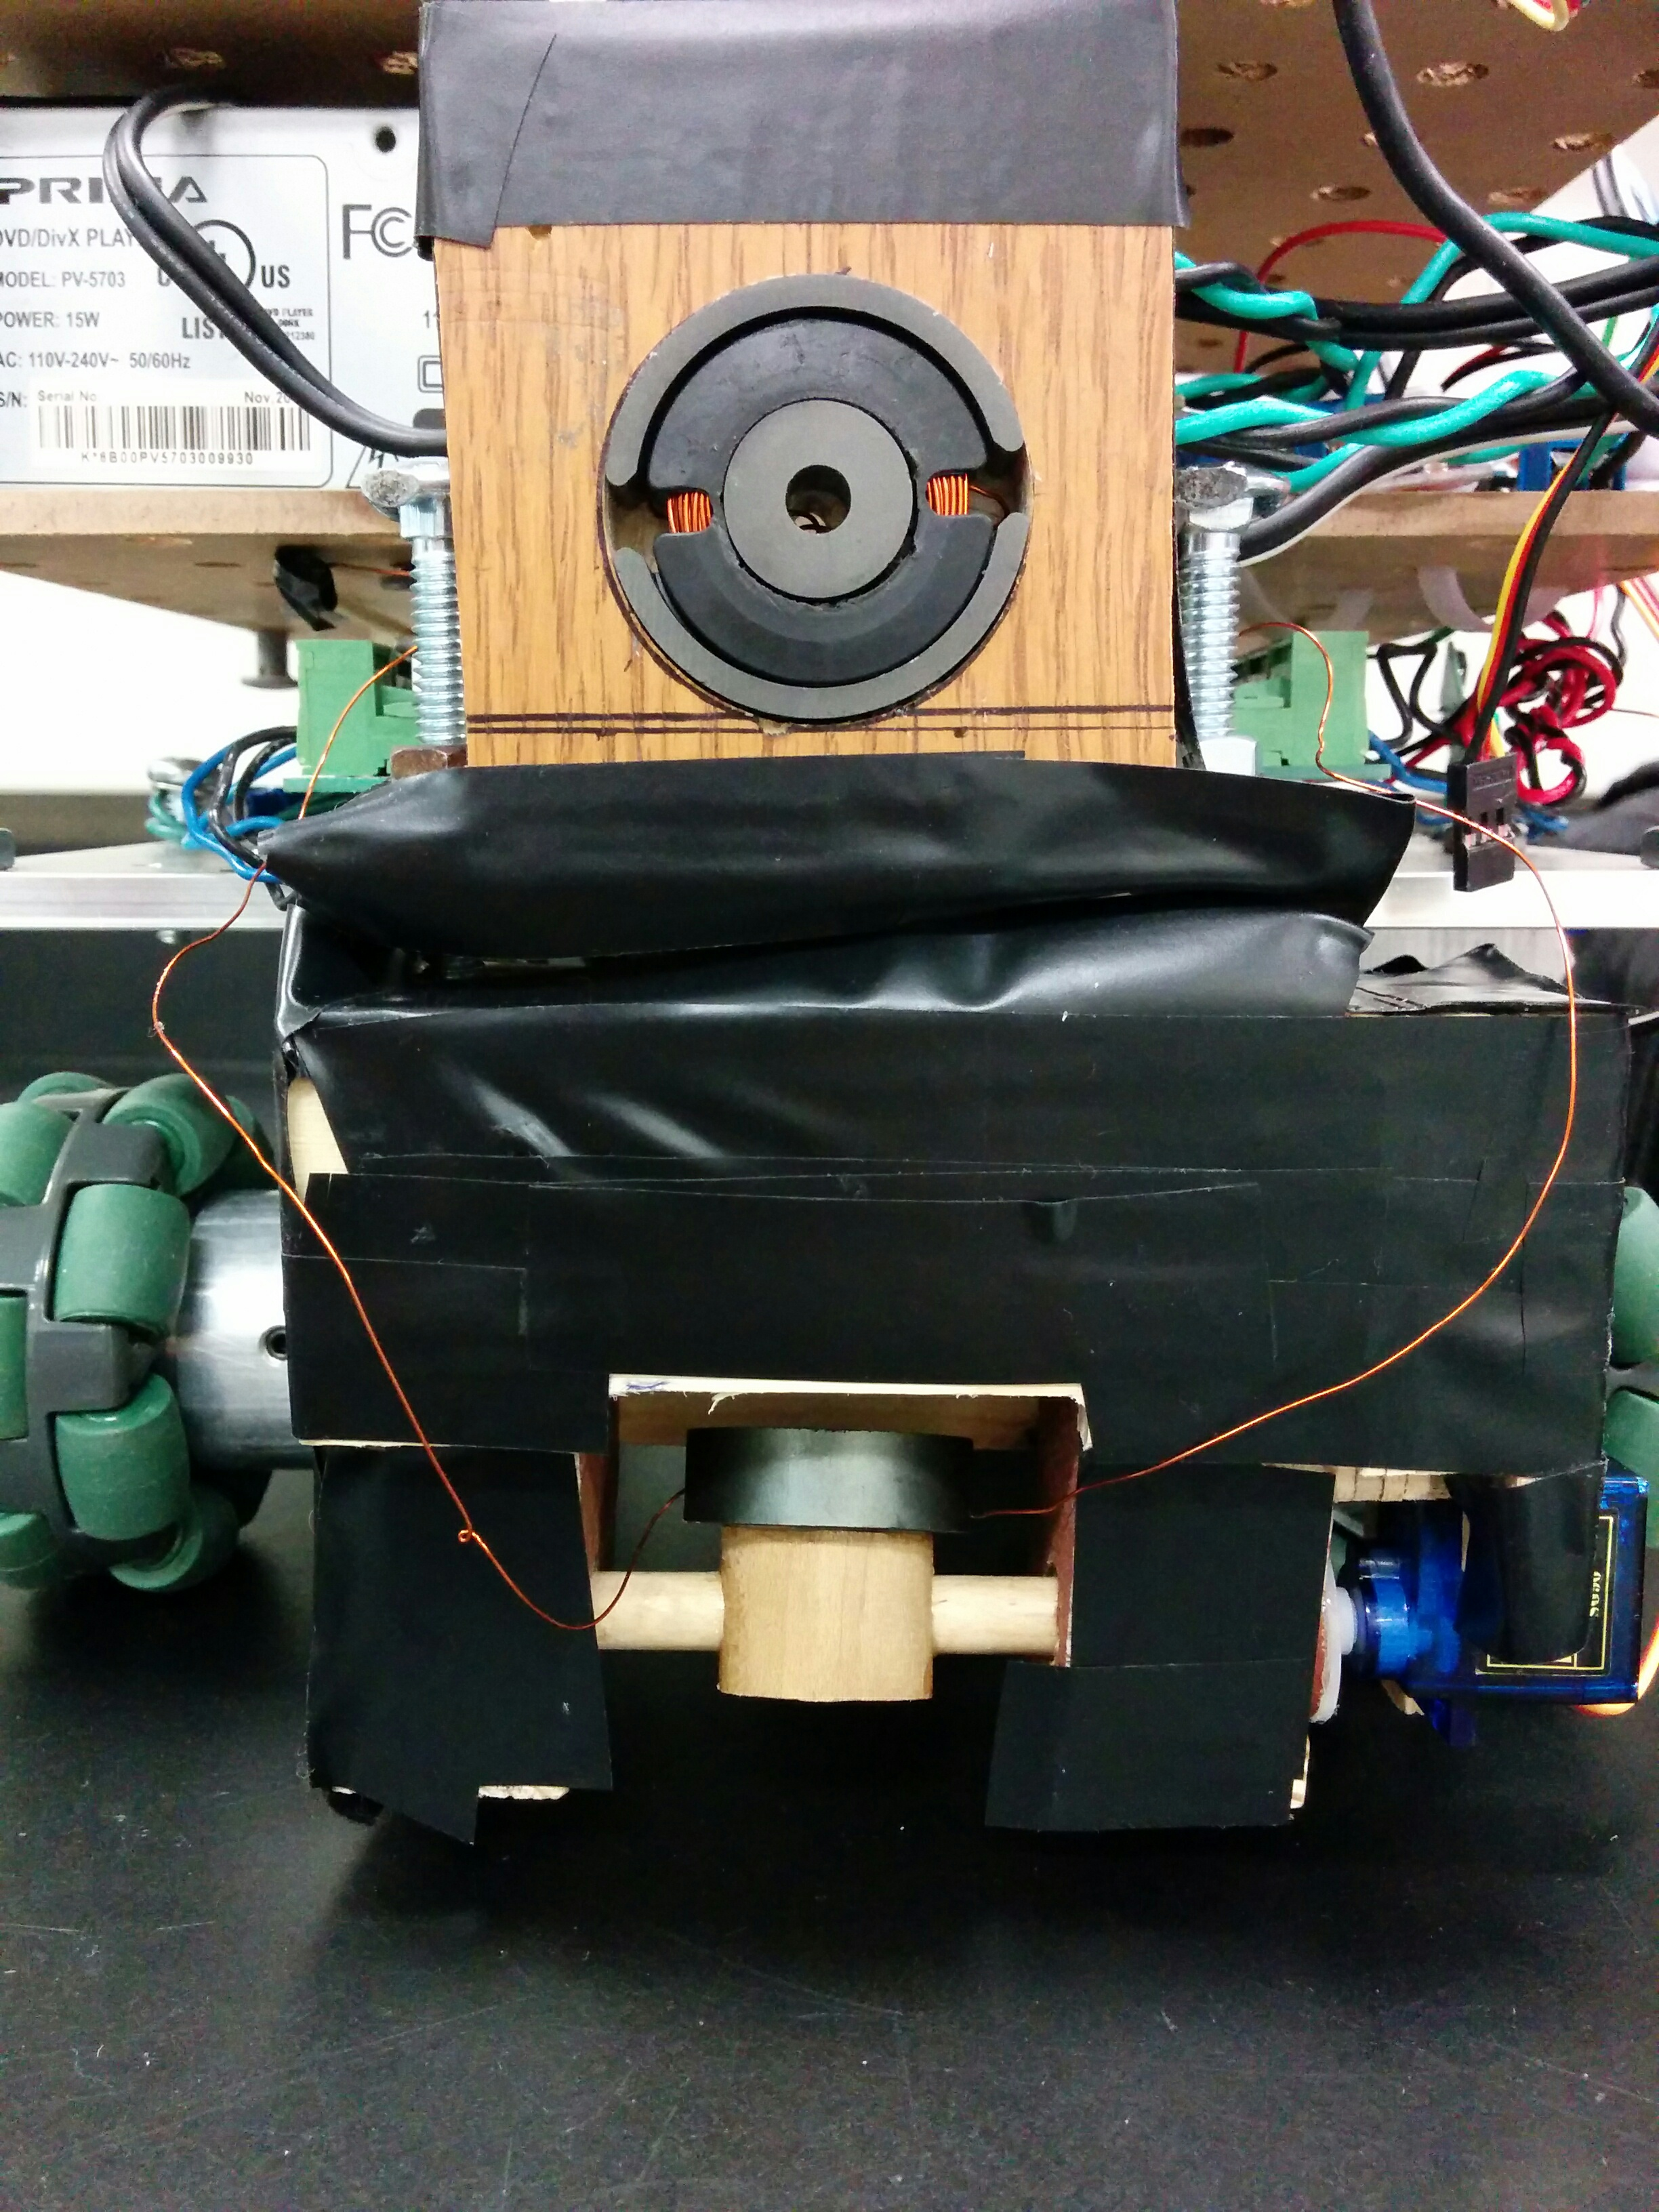
\includegraphics[scale=0.05]{resources/prehenseur_up.jpg}
  \caption{préhenseur en position de conservation du trésor}
  \label{fig:lift_up}
\end{figure}

\section{Transmission et décodage du code manschester}

Afin de transmettre le code manchester entre la station de base et le robot, un module transmetteur et un récepteur de fréquence radio 433 MHz sont utilisés.
Pour ce faire, un microcontrôleur de type Arduino Mega se trouvant à la station de base lit d'abord le code manchester en se synchronisant par interuption
sur le signal de l'horloge, sans le décoder. Par la suite, un port TX est utilisé afin de diffuser en continu le code avec un baudrate de 600 dans le transmetteur
RF. Sur le robot, le récepteur RF est branché sur un port RX avec le même baudrate que le transmetteur. Il suffit alors de lire le contenu du buffer
série 4 fois (4x8 bits) afin d'obtenir les 32 bits du code manchester qui est décodé par la suite sur le Arduino. Le Arduino décode continuellement le
contenu du buffer série.
\paragraph{}
Puisque le signal d'horloge n'est pas transmis, il faut trouver le point de départ en identifiant la séquence de 18 bits fixes de départ
(le signal de données manschester contient deux fois plus de bits que le code original). Une fois cette séquence de départ identifiée,
il suffit de décoder les 14 bits restants. Pour ce faire, les bits sont simplement regroupés en sous-séquences de deux bits.
Une sous-séquence 0-1 signifie un '1' tandis qu'une sous-séquence 1-0 signifie un 0. Tout autre sous-séquence est interprétée comme une erreur et on recommence
l'acquisition du code manchester. Suite à ce décodage, une séquence de 7 bits est obtenue, correspondant au signal ASCII désiré. Si le contenu ne correspond
pas à un code manchester (même nombre de 1 que de 0, 8 bits à "1" de suite suivi d'un bit à "0"), le dernier code manchester valide est
gardé en mémoire jusqu'à ce qu'un autre code valide le remplace. L'ordinateur embarqué peut en tout temps demander le dernier code manchester décodé valide.
